\textbf{PROBLEMA 3}
\vspace{20px}

En el circuito de la figura, los valores de las resistencias son $R_1 = 1\,\Omega$ y $R_2 = 100\,\Omega$. Sin embargo,
desconocemos la fuerza electromotriz de la fuente de tensión y la capacidad del condensador. Suponga en todo
momento que la fuente de tensión es ideal (su resistencia interna es despreciable).

\begin{enumerate}[label=\alph*.]
    \item Suponga que, inicialmente, el condensador está completamente descargado. En un momento determinado,
    situamos el interruptor en la posición $A$, conectando la fuente $\mathcal{E}$ y formando un circuito $RC$ con la
    resistencia $R_1$ y el condensador. Con un osciloscopio, medimos el voltaje entre las placas del condensador
    en función del tiempo, $v_C (t)$ y obtenemos, para los instantes previos y posteriores a la conexión de la
    fuente, la curva de la figura. Sabiendo que cada división del eje vertical representa 5\,V, deduzca la fuerza
    electromotriz de la fuente explicando brevemente su razonamiento.
    \item Desconocemos la capacidad del condensador, pero en el laboratorio solo tenemos condensadores de tres
    capacidades, 5\,$\mu$F, 5\,mF y 5\,F, por lo que el condensador del circuito debe ser alguno de estos tres. Sabiendo
    que cada división del eje horizontal de la gráfica representa 5\,s, deduzca la capacidad del condensador
    empleado en el circuito, explicando brevemente su razonamiento.
    \item Suponga que mantenemos el interruptor en la posición $A$ durante un tiempo muy largo, de modo que
    el condensador se carga por completo. En un instante posterior, al que nos referiremos como $t = 0$,
    cambiamos el interruptor a la posición $B$, desconectando la fuente de tensión y conectando el condensador
    a la resistencia $R_2$. Encuentre la expresión para la corriente que circula por la resistencia $R_2$ en función
    del tiempo para $t > 0$.
    \item Si mantenemos el interruptor en la posición $B$ durante un tiempo indefinido, calcule, por el procedimiento
    que considere más adecuado, la energı́a total que disipa la resistencia $R_2$ entre $t = 0$ y $t\;$\rightarrow$ \infty$.
\end{enumerate}

\begin{center}
    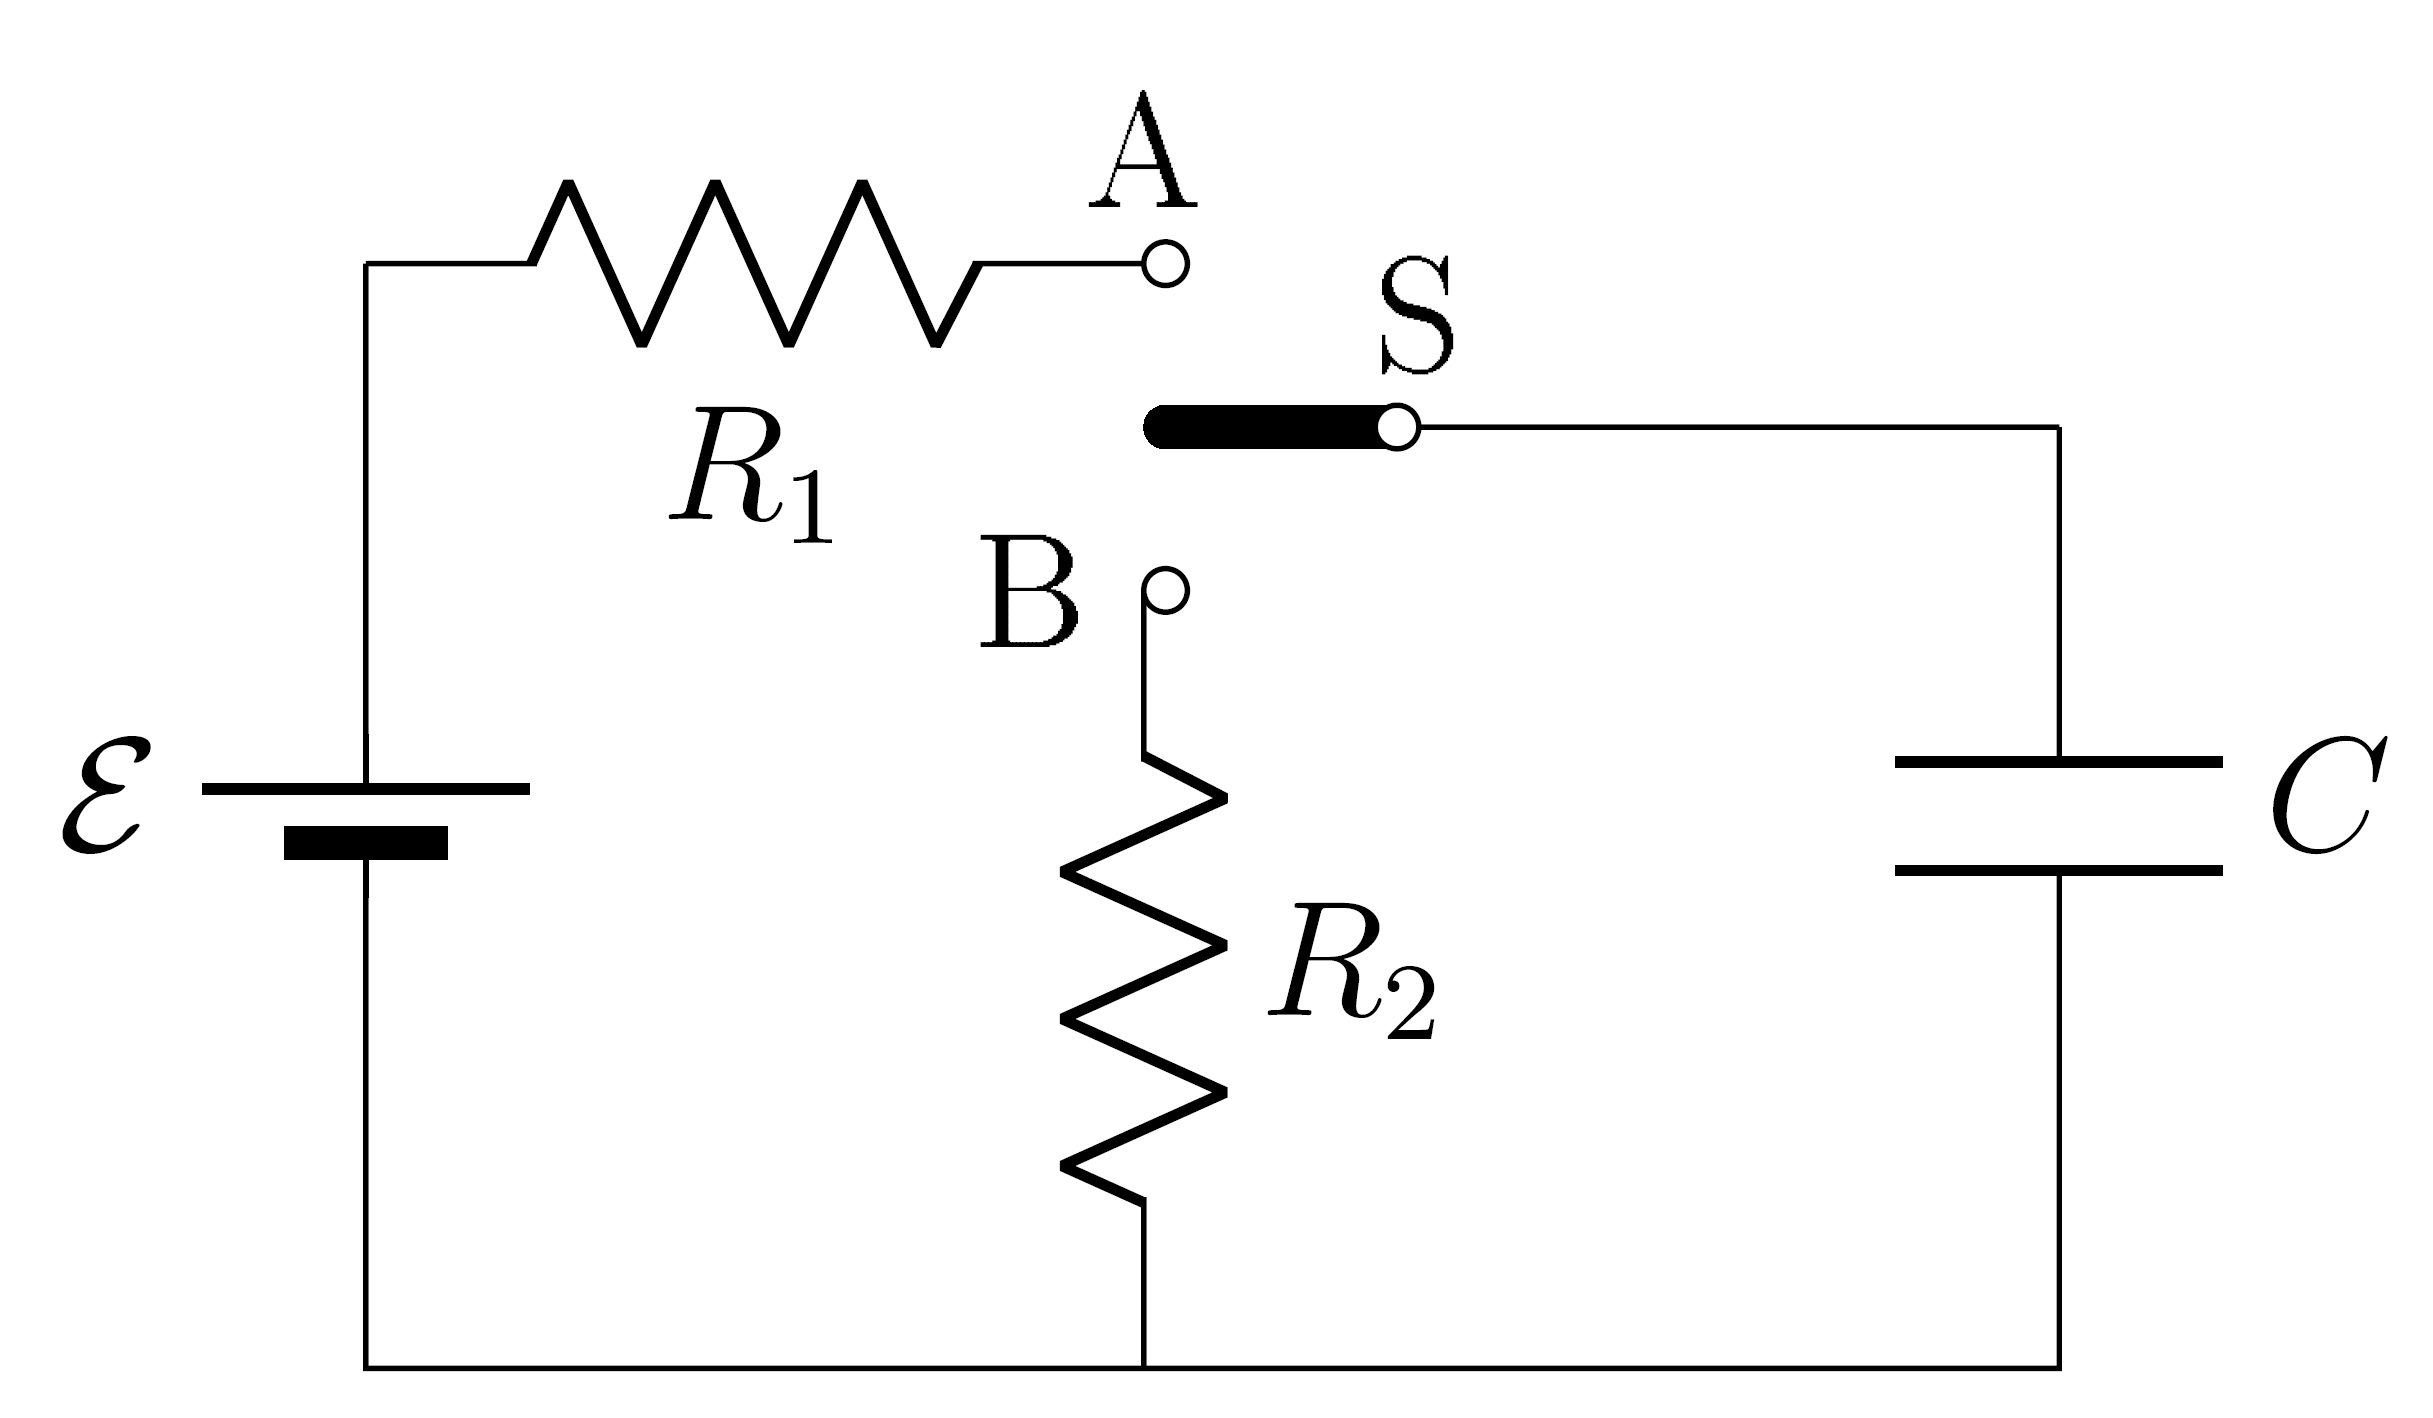
\includegraphics[width=12cm]{files/img3}
\end{center}
\begin{center}
    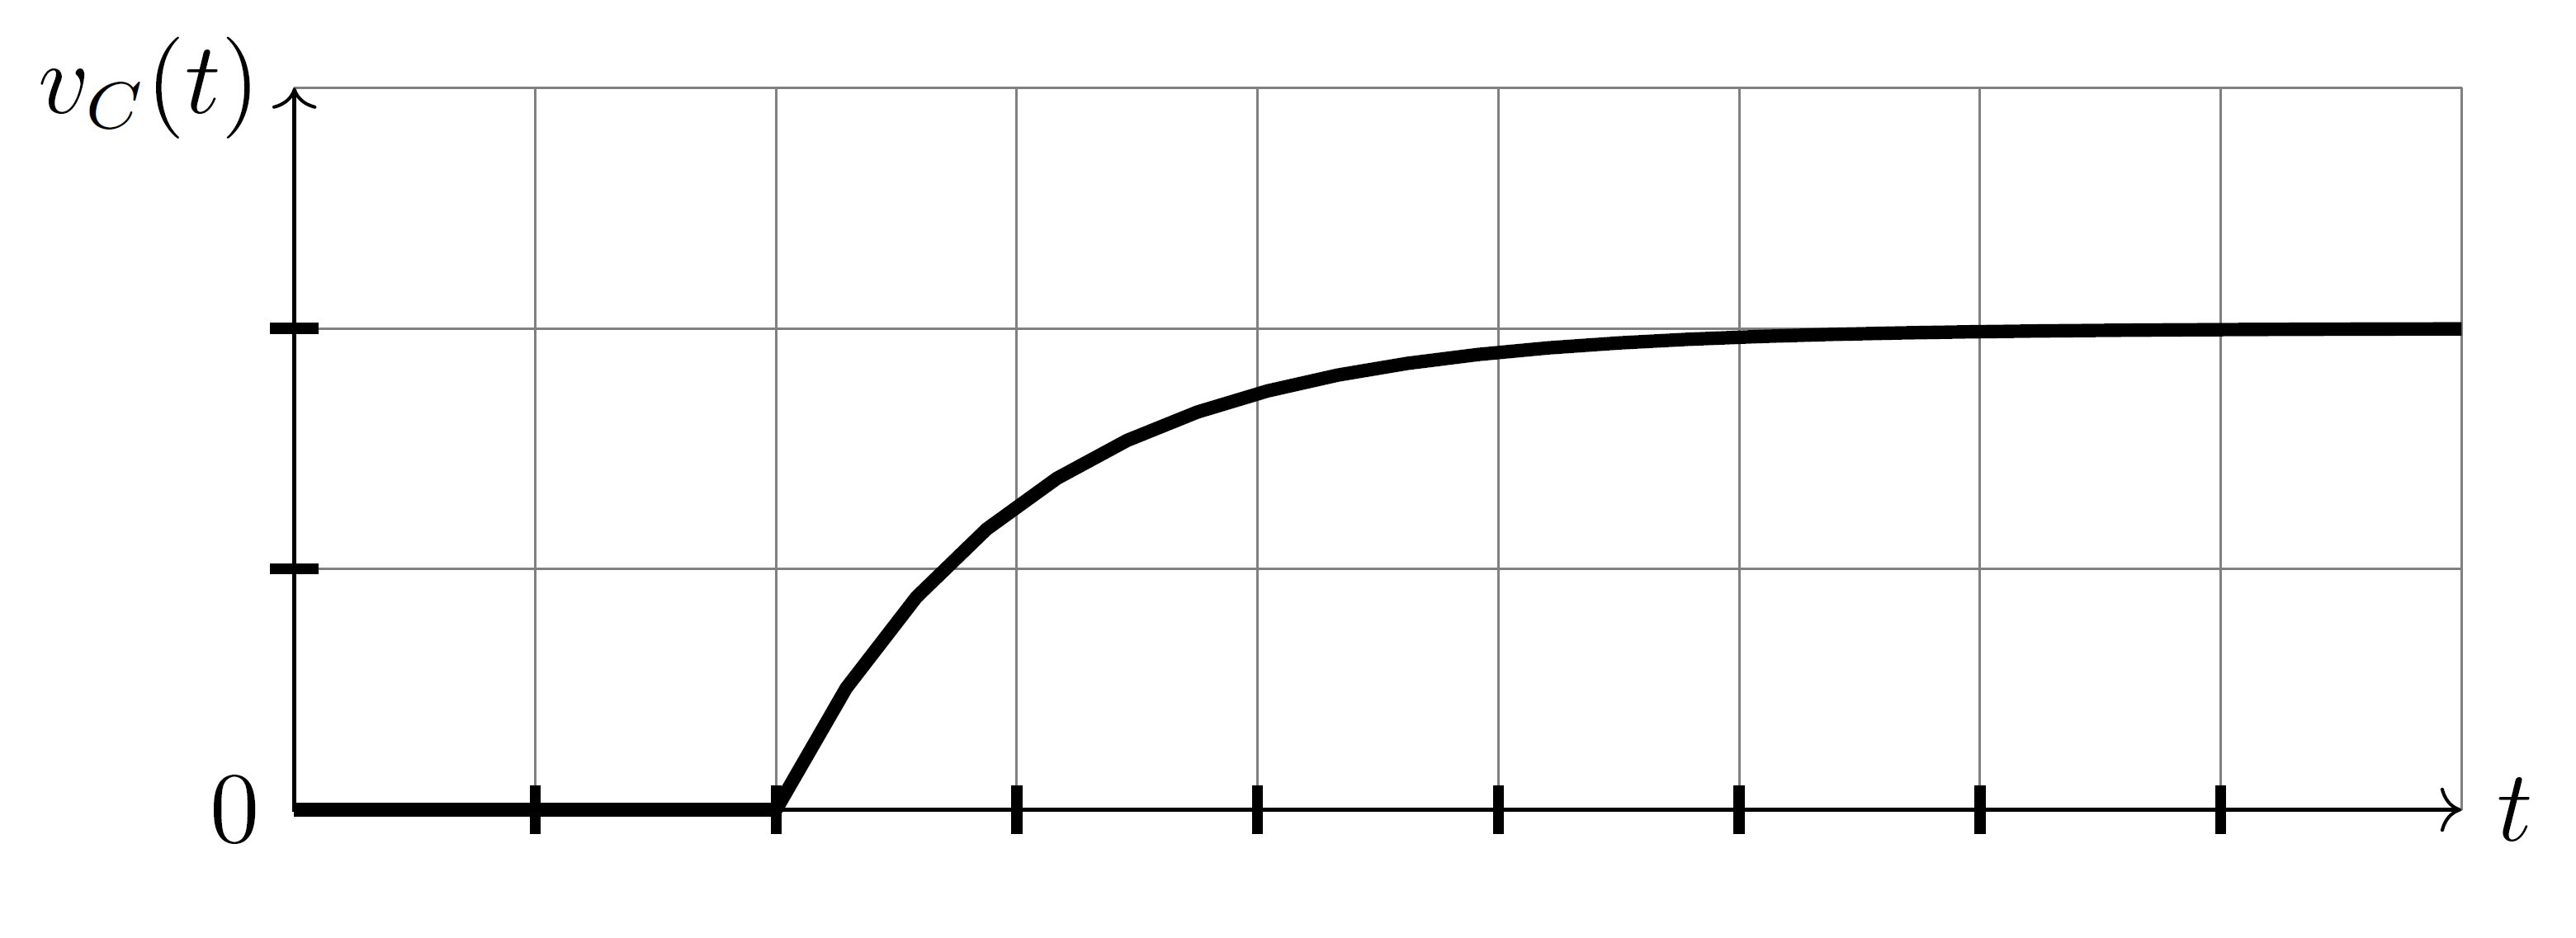
\includegraphics[width=12cm]{files/img4}
\end{center}

\vspace{20px}
\textit{Solución:}
\\